% Intended LaTeX compiler: pdflatex
\documentclass[bigger]{beamer}
\usepackage[utf8]{inputenc}
\usepackage[T1]{fontenc}
\usepackage{graphicx}
\usepackage{longtable}
\usepackage{wrapfig}
\usepackage{rotating}
\usepackage[normalem]{ulem}
\usepackage{amsmath}
\usepackage{amssymb}
\usepackage{capt-of}
\usepackage{hyperref}
\mode<beamer>{\usetheme{Madrid}}
\mode<beamer>{\usepackage{amsmath}}
\usetheme{default}
\author{Konstantinos Papadimos}
\date{}
\title{Presentation draft}
\hypersetup{
 pdfauthor={Konstantinos Papadimos},
 pdftitle={Presentation draft},
 pdfkeywords={},
 pdfsubject={},
 pdfcreator={Emacs 28.2 (Org mode 9.5.5)}, 
 pdflang={English}}
\begin{document}

\maketitle

\section{Introductory stuff, Detectros and Particle physics}
\label{sec:orgb57b208}
\begin{frame}[label={sec:org5e8dae8}]{The CMS Experiment overview}
The CMS detector at the LHC
\begin{figure}[hb]
\centering
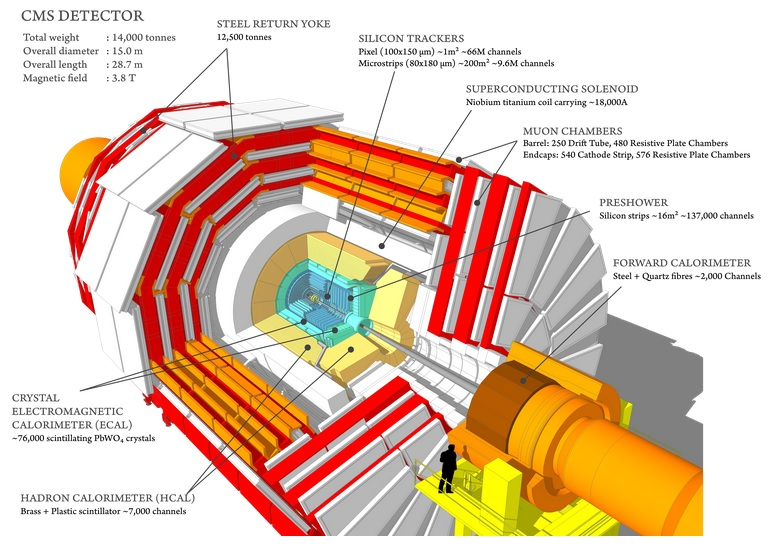
\includegraphics[width=0.7 \textwidth, ext=.png type=jpg]{/home/kpapad/UG_thesis/Thesis/Dissertation/src/figures/cms_detector.jpg}
\end{figure}
\end{frame}

\begin{frame}[label={sec:orgaf36971}]{Coordinates at the CMS}
Given the solenoid geometry of the CMS detector, it is more convenient to use a spherical type of coordinates\(\left(r, \phi, \theta \right)\).
\begin{equation}
\begin{matrix}
p_{x} = P_{T}\cos{\phi} \\
p_{y} = P_{T}\sin{\phi} \\
p_{z} = P_{T}\sinh{\eta}\\
|\vec{P}| = P_{T}\cosh{\eta} 
\end{matrix}
\end{equation}
\(\phi \in \left [ 0, 2\pi \right]\)the azimuthal angle, and \(\eta\in \left [ -\infty, +\infty \right ]\) is defined as:
\begin{equation}
\eta \equiv -\ln{\left [ \tan\left (\frac{\theta}{2} \right ) \right]  }
\end{equation}
\end{frame}

\begin{frame}[label={sec:org9dc6b71}]{Decays \& Resonances}
Not every particle can be detected by the CMS detector(i.e neutrinos)
\begin{columns}
\begin{column}{0.5\columnwidth}
\begin{itemize}
\item Detectable Decay Products \(\rightarrow\) Resonance
\end{itemize}
\begin{center}
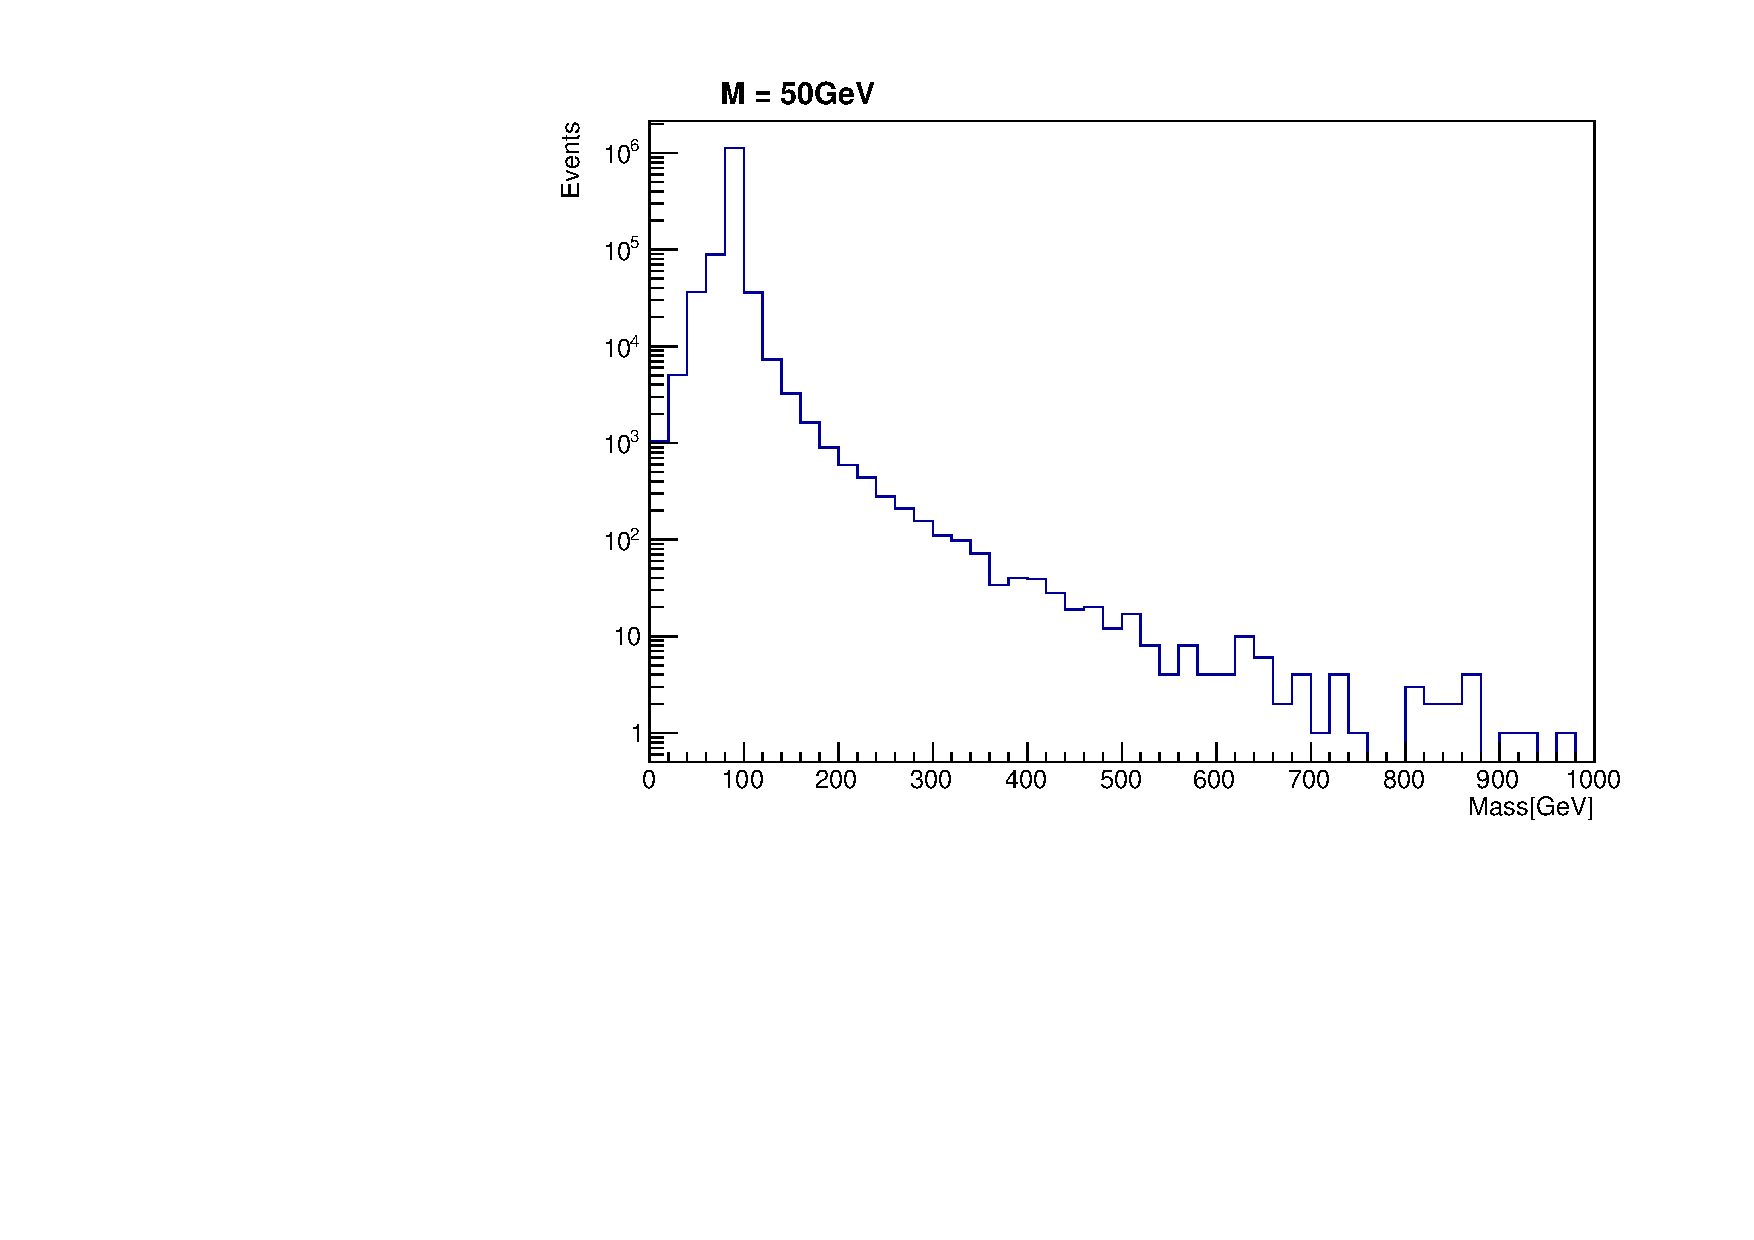
\includegraphics[width=0.8\textwidth]{/home/kpapad/UG_thesis/Thesis/Analysis/out/Plots/DYJetsM50_MassHist.pdf}
\end{center}
\end{column}

\begin{column}{0.5\columnwidth}
\begin{itemize}
\item Non Detectable Decay Products \(\rightarrow\) Not a resonance
\end{itemize}
\begin{center}
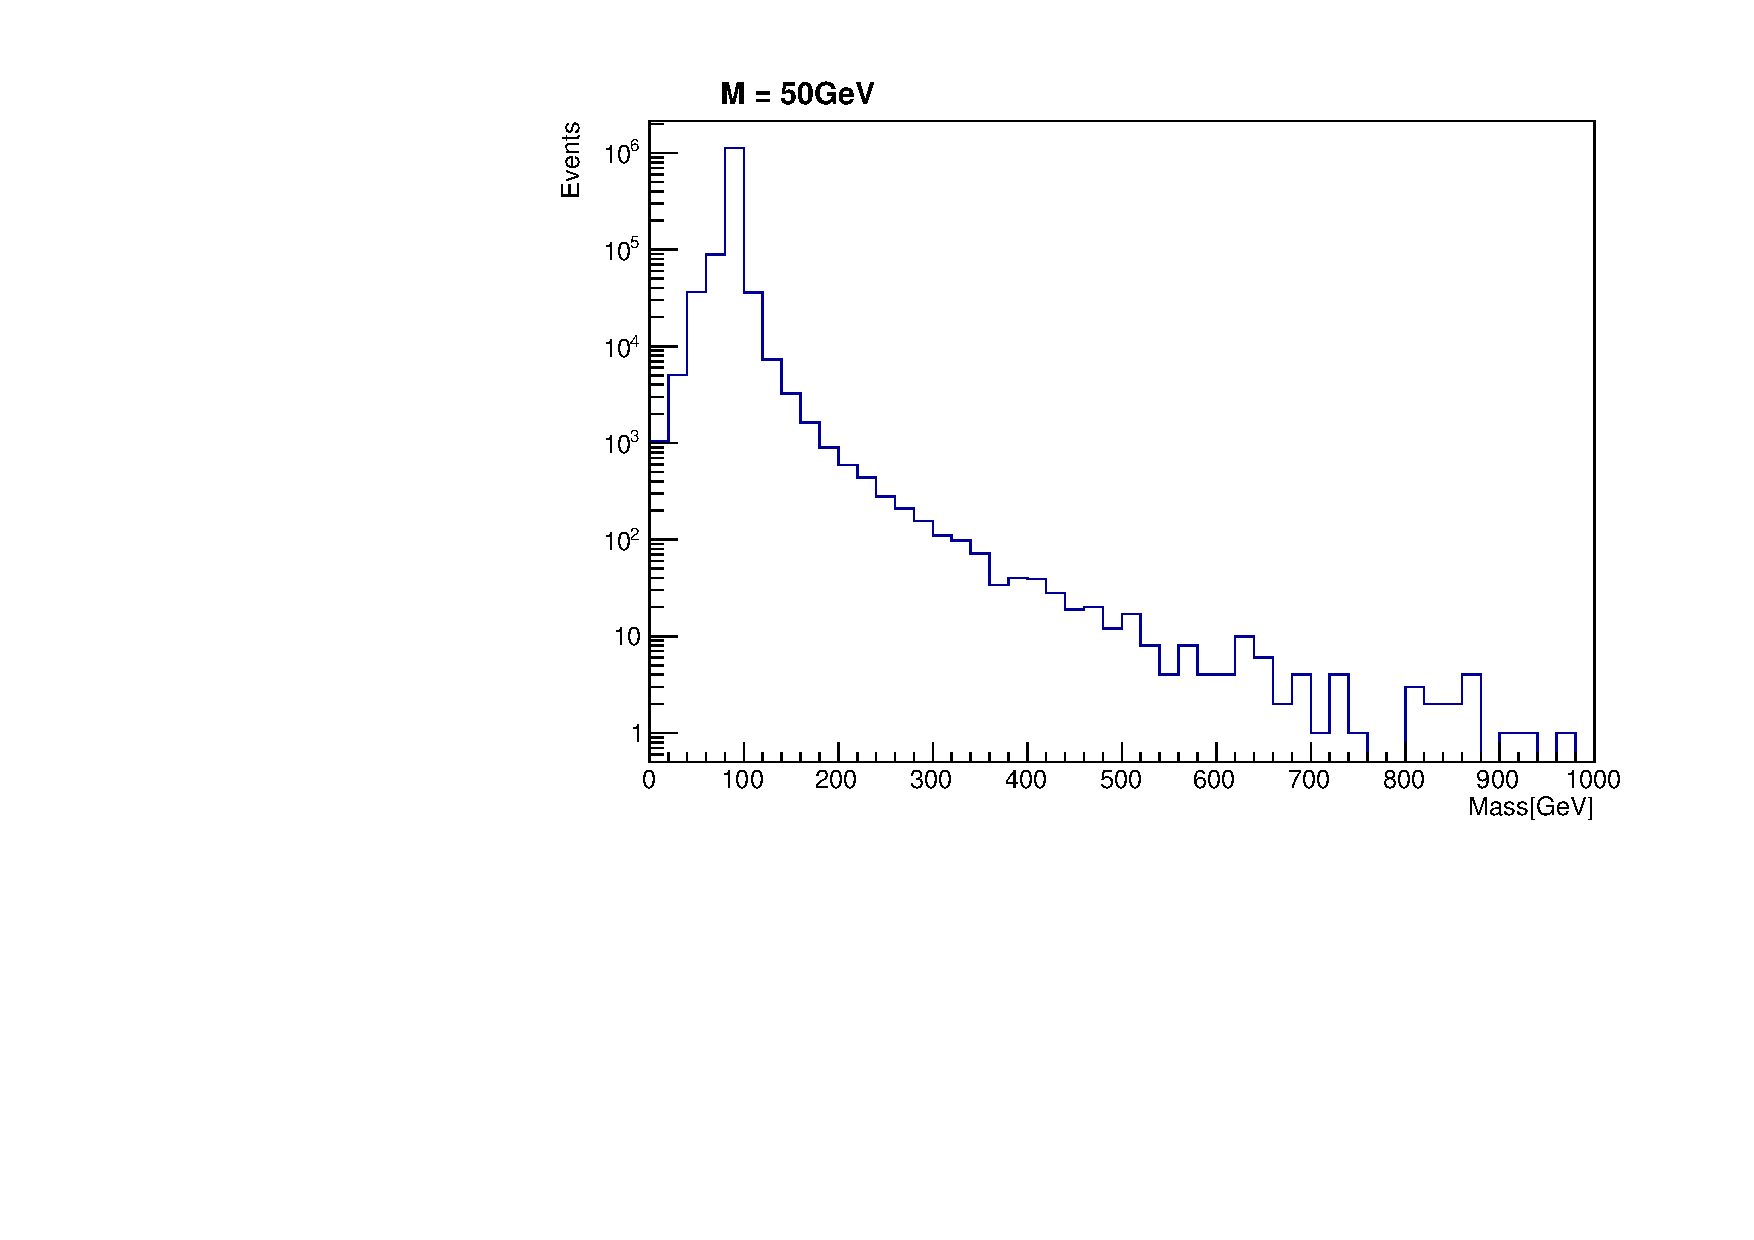
\includegraphics[width=.9\linewidth]{/home/kpapad/UG_thesis/Thesis/Analysis/out/Plots/DYJetsM50_MassHist.pdf}
\end{center}
\end{column}
\end{columns}
\end{frame}

\begin{frame}[label={sec:orgb265b52}]{Calibration and energy scale uncertainties}
\begin{itemize}
\item Calibration process adjusts energy scale and resolution to match well-known resonances (Z boson, J/psi meson) in data and simulation,
\end{itemize}
\begin{itemize}
\item Imperfect agreement due to subdetector complexities and nonlinear effects
\end{itemize}
\begin{block}{How do analysis techniques respond to energy scale uncertainties ?}
Our work will focus on the effects that energy scale uncertainties have, on a traditional fit-based analysis and a more modern Boosted Decision Tree-based analysis, using the generic diobject production process as the working example.
\end{block}
\end{frame}
\section{Analysis techniqies}
\label{sec:org2832127}
\begin{frame}[label={sec:org0c6299e}]{BDT 1: Supervised Learning}
\alert{Supervised learning}:
\begin{itemize}
\item The model is trained using training data
\item The trained model is tested using testing data
\item If we like the resulting model, we apply it!
\end{itemize}

\alert{but what is this model?}
\begin{itemize}
\item A function that given the input feautres x, it returns the probability x beeing class A
\item The goal of the training is to minimize the difference between the predicted output \(y_{i} \in [0, 1]\) and the real output \(\hat{y_{i}} = 0\text{ class B, or }\hat{y_{i}} = 1\text{ class A}\)
\end{itemize}
\end{frame}
\begin{frame}[label={sec:org600b6c5}]{BDT 2a: Boosted decision trees}
In this study the model of choice is Boosted Decision Trees(BDT).
\begin{itemize}
\item It classifies data using decision tree models
\end{itemize}
\begin{figure}[h]
\centering
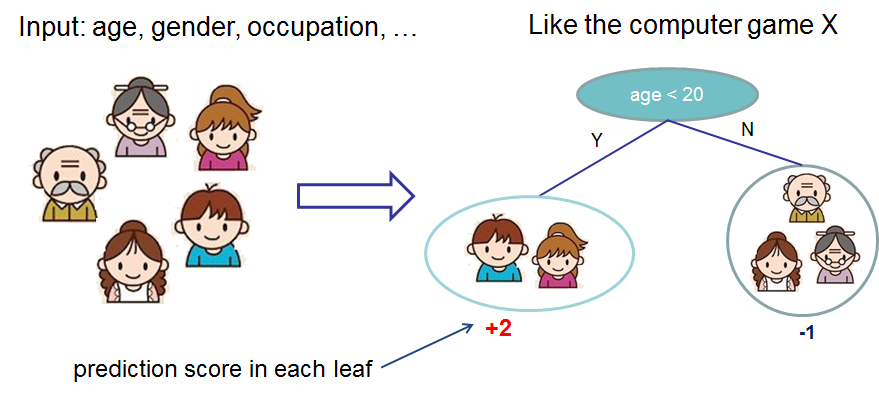
\includegraphics[width=0.85 \textwidth, ext=.png type=png]{/home/kpapad/UG_thesis/Thesis/Dissertation/Presentation/figures/cart.png}
\end{figure}
\end{frame}
\begin{frame}[label={sec:org7c60e44}]{BDT 2b: Boosted Decision Trees}
Usually only one tree is not power full enough --> Use  more trees in additive manner(Boosting)
\begin{figure}[h]
\centering
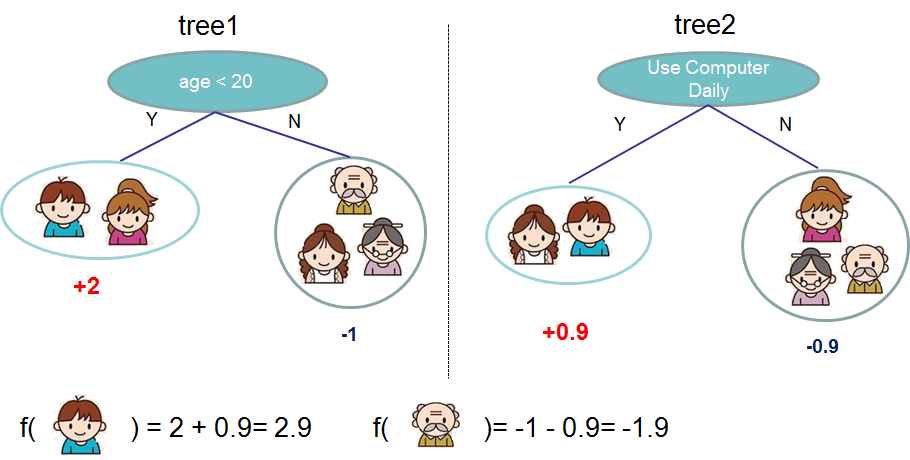
\includegraphics[width=0.85 \textwidth, ext=.png type=png]{/home/kpapad/UG_thesis/Thesis/Dissertation/Presentation/figures/twocart.png}
\end{figure}
\end{frame}
\begin{frame}[label={sec:org3ab0a17}]{BDT 3a: Signal from Background Separation}
\alert{In our case}:
\begin{itemize}
\item Signal: a resonant decay Y->xx
\item Background: a non resonant process
\end{itemize}
\alert{How to separate them?}
\begin{itemize}
\item Plot the number of Signal and Background events per BDT score --> BDT histogram
\end{itemize}
\end{frame}
\begin{frame}[label={sec:org3be83ed}]{BDT 3b: Signal from background separation}
Where should we place the cut in order to accpet most most of the  signal while rejecting most of background?
\begin{figure}[hb]
\centering
\includegraphics[page=2, width=0.85 \textwidth, ext=.png type=jpg]{/home/kpapad/UG_thesis/Thesis/Bdt/out/Plots/WPhiJets_M60M5080DeltasPConf12BDTplot.pdf}
\end{figure}
\end{frame}
\begin{frame}[label={sec:org59e9c82}]{Fit based signal from background separation}
Fit the mass spectrum \ldots{}
\begin{figure}[hb]
\centering
\includegraphics[page=2, width=0.5 \textwidth, ext=.png type=jpg]{/home/kpapad/UG_thesis/Thesis/Analysis/src/WPhiJets_M60M5080_SampleFitWArrows.pdf}
\end{figure}
\end{frame}
\begin{frame}[label={sec:orgc633832}]{Fit based signal from background separation}
\ldots{} and decompose it to a background component \ldots{}
\begin{figure}[hb]
\centering
\includegraphics[page=3, width=0.5 \textwidth, ext=.png type=jpg]{/home/kpapad/UG_thesis/Thesis/Analysis/src/WPhiJets_M60M5080_SampleFitWArrows.pdf}
\end{figure}
\end{frame}
\begin{frame}[label={sec:org6f53951}]{Fit based signal from background separation}
\ldots{} and a signal component
\begin{figure}[hb]
\centering
\includegraphics[page=4, width=0.5 \textwidth, ext=.png type=jpg]{/home/kpapad/UG_thesis/Thesis/Analysis/src/WPhiJets_M60M5080_SampleFitWArrows.pdf}
\end{figure}
\end{frame}
\begin{frame}[label={sec:orge08089d}]{Fit based signal from background separation}
Then we can count the signal and background events, in a region of interest \(I\):
\begin{align}
O &= \int_{I} observation(x) dx \\
B &= \int_{I} bkg(x) dx\\
S &= O - B
\end{align}
\end{frame}
\begin{frame}[label={sec:org437e7ce}]{Statistical interpretation of results}
\alert{Are the signal events we counted, statistically significant?}
\begin{itemize}
\item We use the following metric:
\end{itemize}
\begin{equation}
\text{Significance} = \frac{Signal}{\sqrt{Background}}
\end{equation}
\begin{itemize}
\item The selected regions of interest both in BDT and Fit based analysis, are those that maximize the significance.
\end{itemize}
\end{frame}

\section{Analysis1: General Stuff}
\label{sec:org706c799}
\begin{frame}[label={sec:org6483296}]{Searches for \(Y \rightarrow XX\)}
\begin{columns}
\begin{column}{0.5\columnwidth}
Search for heavy \(Y \rightarrow XX\)
\begin{itemize}
\item Mass range from 100GeV up to 300GeV
\end{itemize}
\end{column}
\begin{column}{0.5\columnwidth}
Search for light \(Y \rightarrow XX\)
\begin{itemize}
\item Mass range from 50GeV up to 70GeV
\end{itemize}
\end{column}
\end{columns}
\end{frame}
\begin{frame}[label={sec:org357ba87}]{The \(Y \rightarrow XX\) channel}
The specific characteristics(mass etc.) of each dataset  is different but the main idea is the same
\begin{itemize}
\item Use a non resonant process for background
\item Use a resonant process for signal
\item Separate signal from background
\item Apply energy scale uncertainties to signal
\item Separate again
\item Compare the nominal case with the smeared cases
\end{itemize}
\end{frame}
\begin{frame}[label={sec:org232b624}]{The \(Y \rightarrow XX\) channel: Background}
\begin{itemize}
\item Drell-Yan process
\end{itemize}
\end{frame}

\begin{frame}[label={sec:org8ad639b}]{The \(Y \rightarrow XX\) channel: Signal}
\begin{itemize}
\item W \(\Phi\) --> ll
\end{itemize}
\end{frame}

\begin{frame}[label={sec:orgbec14de}]{Energy scale uncertainties}
To smear the data by \(x\%\),
\begin{itemize}
\item iterate over every signal event
\item multiply each \(P_{T}\) by a number sampled from a Gaussian distribution of \(\mu = 1\) and \(\sigma = x/100\)
\end{itemize}
\end{frame}
\section{Light mass search}
\label{sec:orgcb764b8}
\begin{frame}[label={sec:orgd9d9839}]{Search for light \(Y \rightarrow XX\)}
We will study the following smearing cases:
\begin{itemize}
\item \(0\%\)(Nominal case)
\item \(5\%\)
\item \(7\%\)
\item \(10\%\)
\item \(12\%\)
\end{itemize}
The number of events of the application set are quite low --> smearing has a significant effect real quick 
\end{frame}
\begin{frame}[label={sec:org298e900}]{Fit based approach: The application set}
\begin{columns}
\begin{column}{0.5\columnwidth}
\begin{itemize}
\item Signal events: 3K
\item Background events: 30K
\end{itemize}
\end{column}
\begin{column}{0.5\columnwidth}
\begin{figure}[h]
\centering
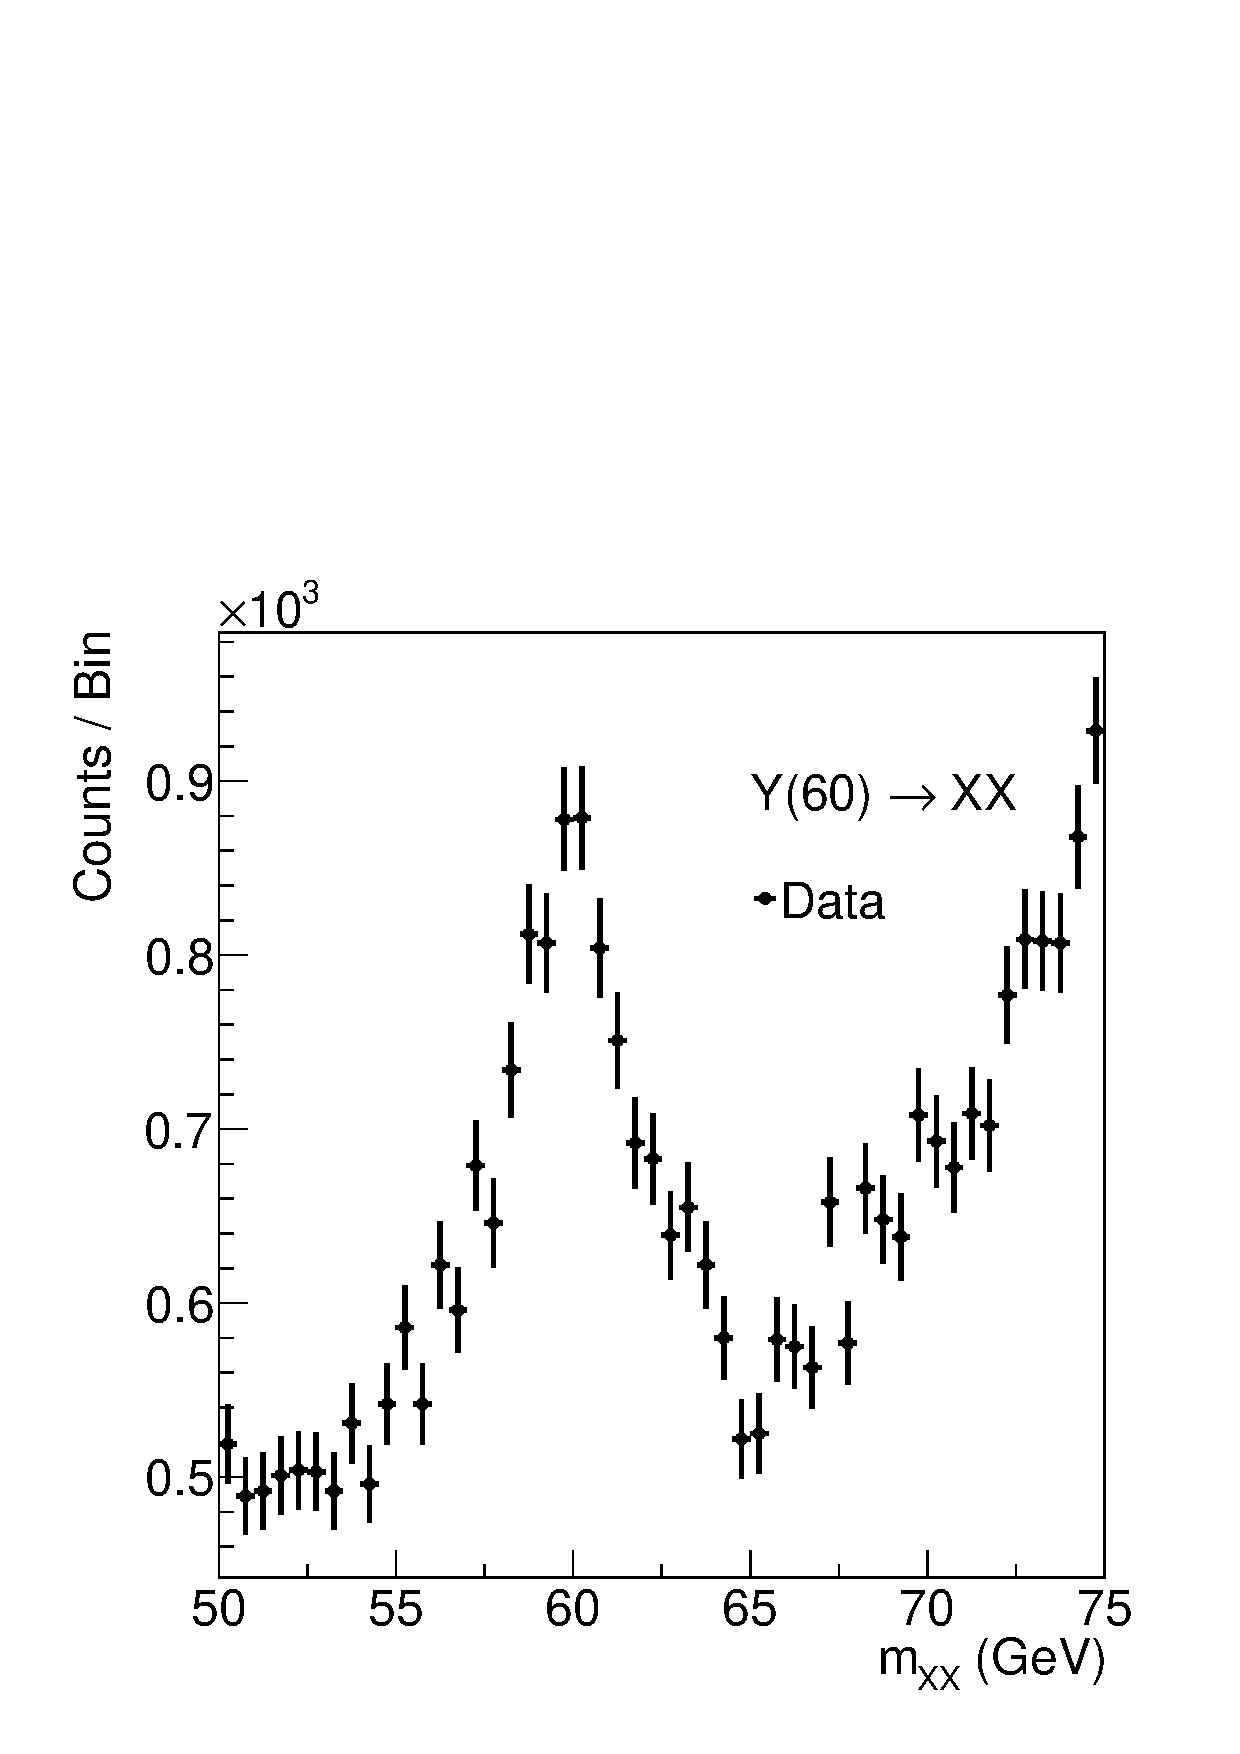
\includegraphics[page=1,width=\textwidth]{/home/kpapad/UG_thesis/Thesis/Analysis/out/Plots/WPhiJets_M60M5080_Application_MassSpectrum.pdf}
\end{figure}
\end{column}
\end{columns}
\end{frame}
\begin{frame}[label={sec:orgd0dde85}]{Fit based approach: Background Fitting}
\begin{columns}
\begin{column}{0.5\columnwidth}
\begin{itemize}
\item To simplify things a bit, we fit the background sepratelly
\item The background shape is kept constant throughout the fits
\item Shape: \(\alpha + \beta x + \gamma x^2 + \delta x^3\)
\end{itemize}
\end{column}
\begin{column}{0.5\columnwidth}
\begin{figure}[h]
\centering
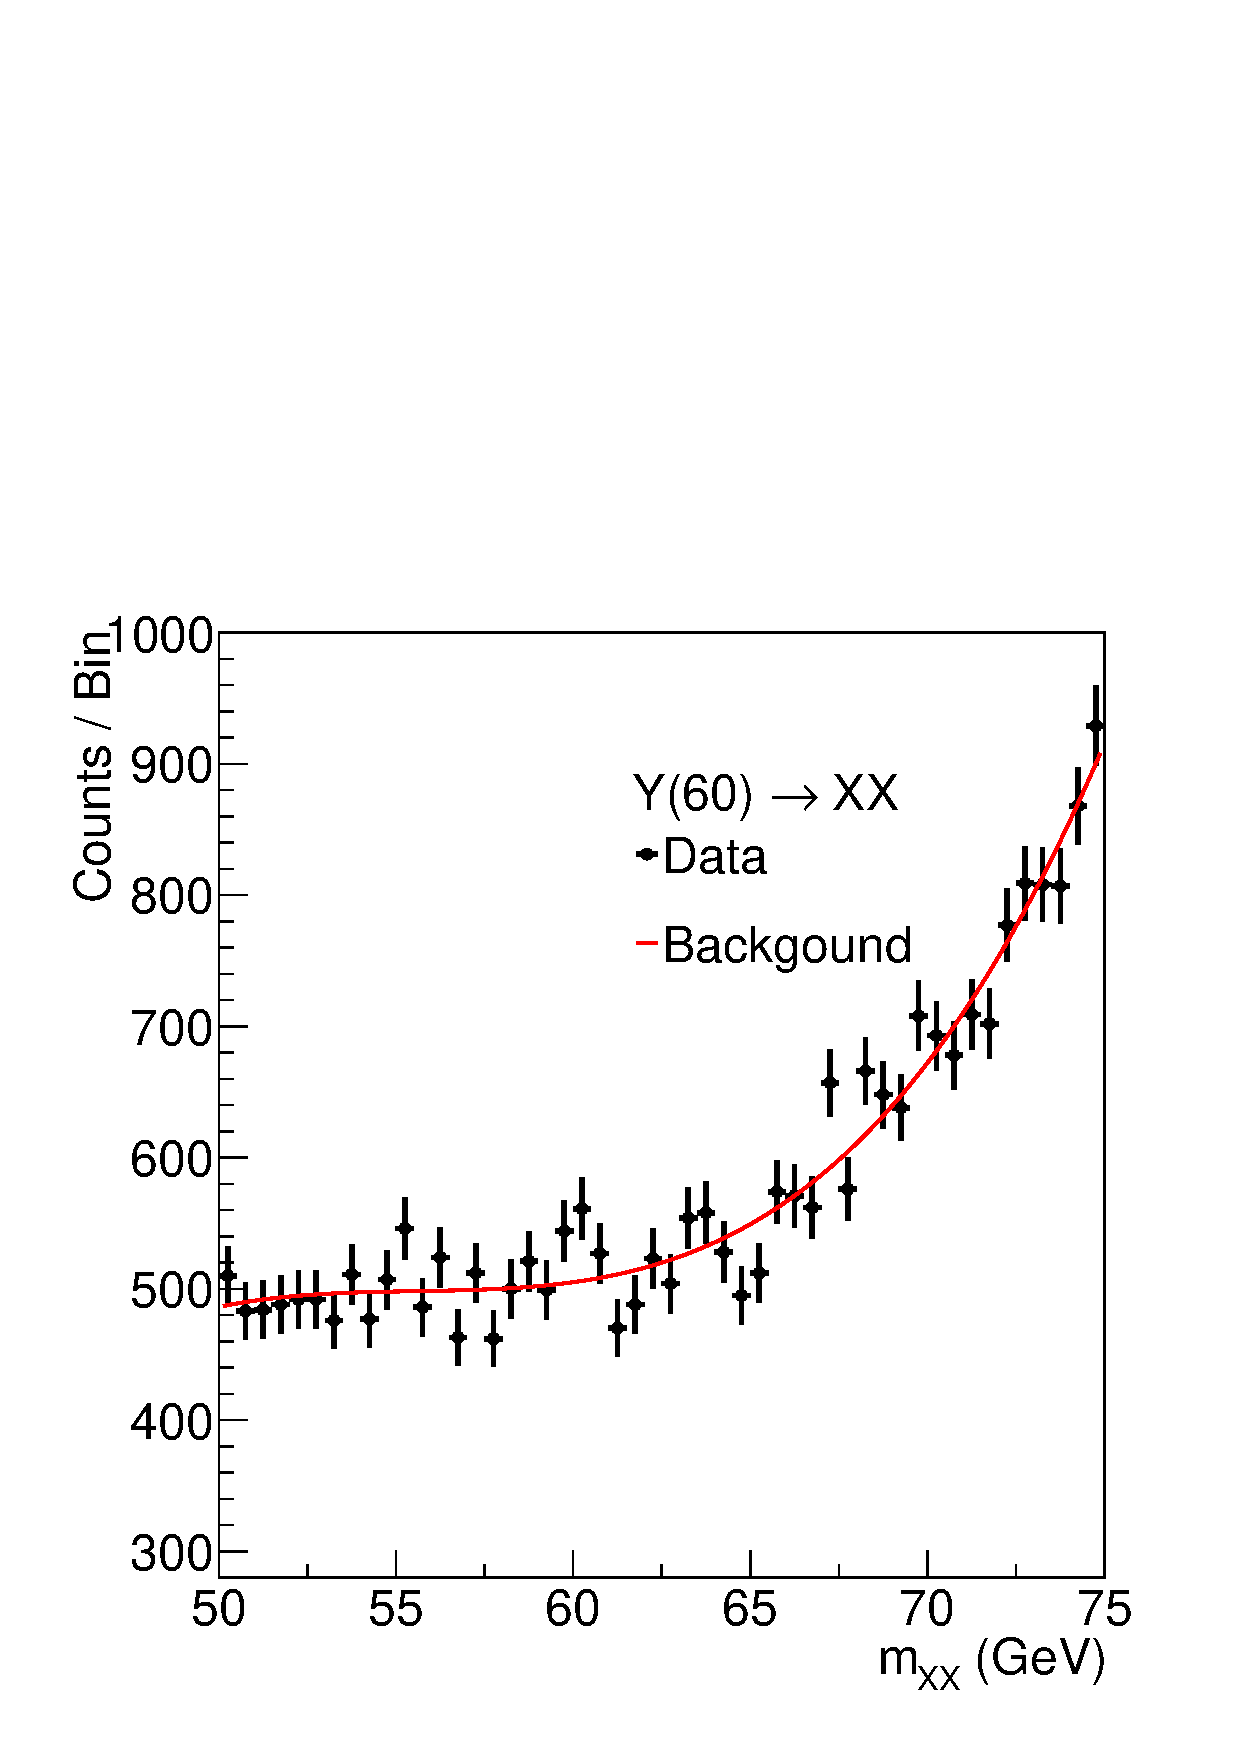
\includegraphics[page=1,width=\textwidth]{/home/kpapad/UG_thesis/Thesis/Analysis/out/Plots/WPhiJets_M60M5080_Application_bkgonly_Fit.pdf}
\end{figure}
\end{column}
\end{columns}
\end{frame}

\begin{frame}[label={sec:org6104694}]{Fit based approach: Signal Fitting}
Then we proceed and fit the signal
\begin{columns}
\begin{column}{0.5\columnwidth}
\begin{figure}[h]
\centering
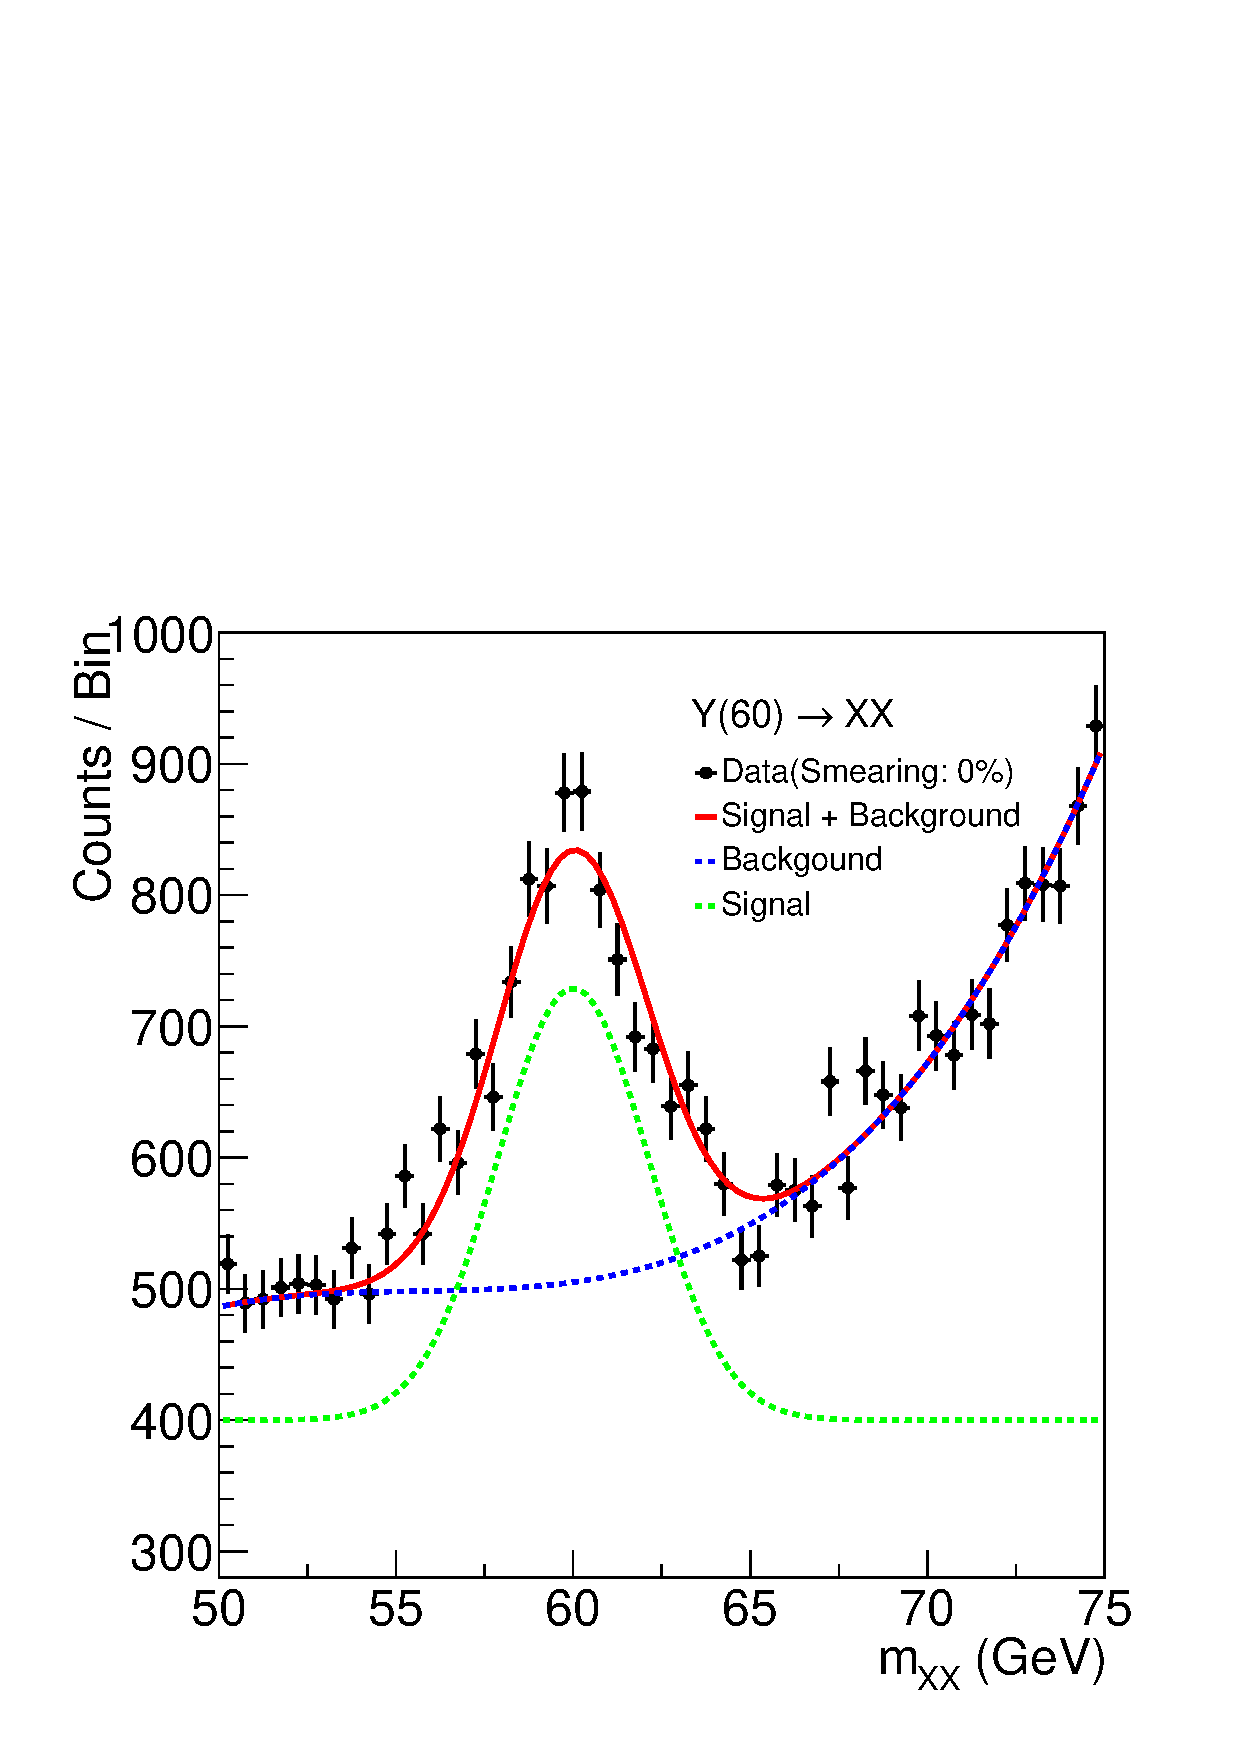
\includegraphics[page=1,width=\linewidth]{/home/kpapad/UG_thesis/Thesis/Analysis/src/WPhiJets_M60M5080_FitALL.pdf}
\end{figure}
\end{column}

\begin{column}{0.5\columnwidth}
\begin{figure}[h]
\centering
\includegraphics[page=2,width=\linewidth]{/home/kpapad/UG_thesis/Thesis/Analysis/src/WPhiJets_M60M5080_FitALL.pdf}
\end{figure}
\end{column}
\end{columns}
\end{frame}

\begin{frame}[label={sec:orgdfa3878}]{Fit based approach: Signal Fitting}
\begin{columns}
\begin{column}{0.5\columnwidth}
\begin{figure}[h]
\centering
\includegraphics[page=3,width=\linewidth]{/home/kpapad/UG_thesis/Thesis/Analysis/src/WPhiJets_M60M5080_FitALL.pdf}
\end{figure}
\end{column}

\begin{column}{0.5\columnwidth}
\begin{figure}[h]
\centering
\includegraphics[page=4,width=\linewidth]{/home/kpapad/UG_thesis/Thesis/Analysis/src/WPhiJets_M60M5080_FitALL.pdf}
\end{figure}
\end{column}
\end{columns}
\end{frame}

\begin{frame}[label={sec:org9e447df}]{Fit based approach: Signal Fitting}
Any further smearing will make the signal indistiguishable!
\begin{figure}[h]
\centering
\includegraphics[page=5,width=0.55\textwidth]{/home/kpapad/UG_thesis/Thesis/Analysis/src/WPhiJets_M60M5080_FitALL.pdf}
\end{figure}
\end{frame}

\begin{frame}[label={sec:org9467c4b}]{Fit based approach: Signal from background separation}
Working in the nominal case, we find the region that yields the best significance, by scanning the ranges \(m=\pm \frac{n}{2}\sigma\text{, }n=1, 2, 3, 4, 5, 6\) 
\begin{figure}[h]
\centering
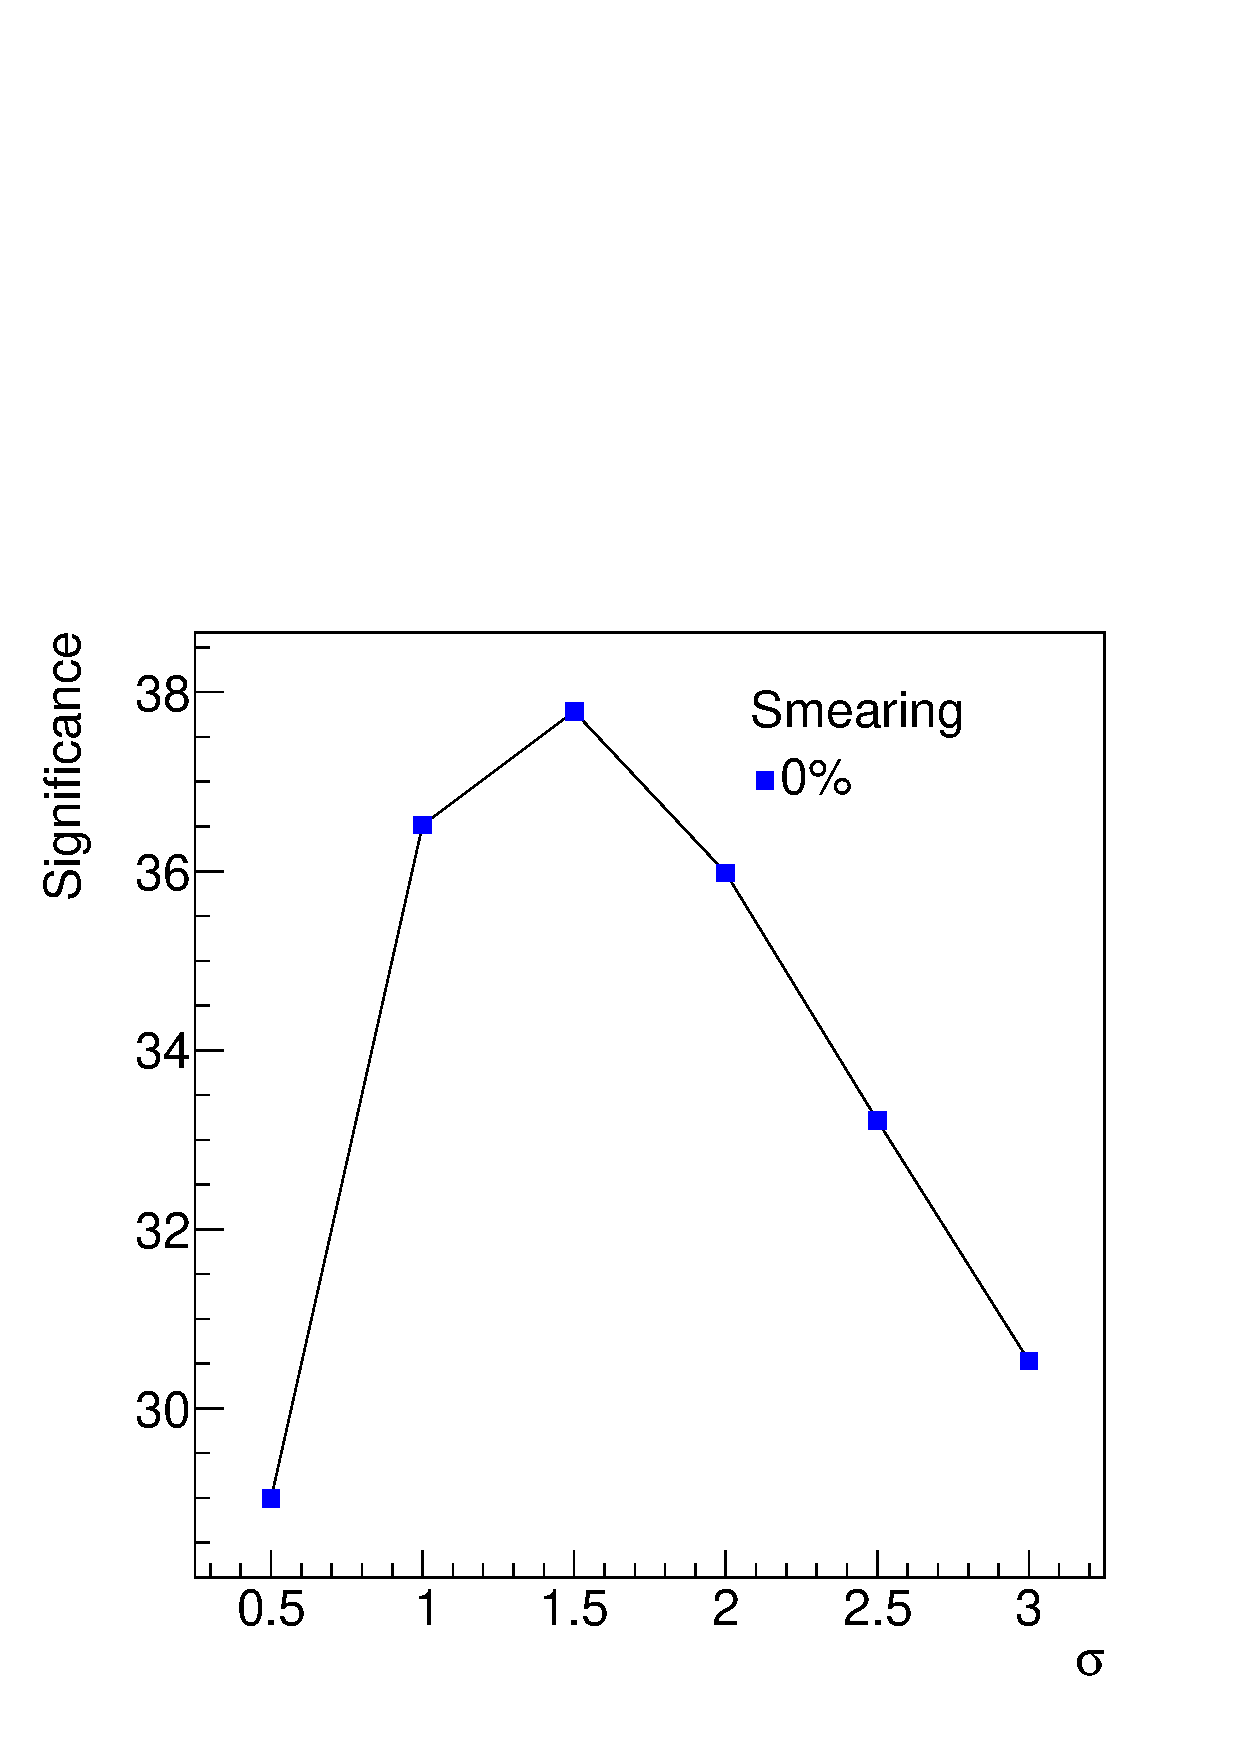
\includegraphics[page=1,width=0.45\linewidth]{/home/kpapad/UG_thesis/Thesis/Analysis/src/WPhiJets_M60M5080_Significance0.pdf}
\end{figure}
\end{frame}
\begin{frame}[label={sec:orge81c0e0}]{Fit based approach: Signal from background separation}
The region of interest that yields the best significance is the \(\pm 1.5\sigma\). There are two ways to interpret this.
\begin{columns}
\begin{column}{0.5\columnwidth}
\begin{itemize}
\item interpret \(\sigma\) as the the spread of the nominal case --> fixed window
\item interpret \(\sigma\) as the the spread of each  cases --> adaptive window
\end{itemize}
\end{column}
\begin{column}{0.5\columnwidth}
\begin{figure}[h]
\centering
\includegraphics[page=3,width=0.8\linewidth]{/home/kpapad/UG_thesis/Thesis/Bdt/src/WPhiJets_M60M5080_Significance.pdf}
\end{figure}
\end{column}
\end{columns}
\end{frame}
\begin{frame}[label={sec:org0b374f4}]{BDT approach 1: Feature space}
\alert{What features of the dataset are best for the classification task?}
\begin{figure}[h!]
\centering
\includegraphics[page=1,width=0.9\textwidth]{/home/kpapad/UG_thesis/Thesis/Analysis/out/Plots/WPhiJets_M60M5080DeltasVarsPlots.pdf}
\end{figure}
\end{frame}
\begin{frame}[label={sec:org2c02496}]{BDT approach1a: Feature space}
\begin{figure}[h!]
\centering
\includegraphics[page=2,width=0.9\textwidth]{/home/kpapad/UG_thesis/Thesis/Analysis/out/Plots/WPhiJets_M60M5080DeltasVarsPlots.pdf}
\end{figure}
\end{frame}

\begin{frame}[label={sec:org41d6c8b}]{BDT approach 2: The model}
\begin{columns}
\begin{column}{0.5\columnwidth}
\begin{itemize}
\item Trained with approximately 3K events
\item To examine overfitting we compare the ratio of training events to testing for each bdt score
\end{itemize}
\end{column}
\begin{column}{0.5\columnwidth}
  \begin{figure}[h!]
\centering
\includegraphics[page=5, width=\textwidth]{/home/kpapad/UG_thesis/Thesis/Bdt/out/Plots/WPhiJets_M60M5080DeltasPConf13BDTplot.pdf}
\end{figure}
\end{column}
\end{columns}
\end{frame}

\section{Results}
\label{sec:orgc2b8f11}
\begin{frame}[label={sec:org919ff68}]{Results 1}
Compare the BDT and FIt in terms of significance and robustness. Comment that even though fit based achieves a higher significance in the 0 smearing case, it is not as robust as bdt, it completelly fails at extreme cases of smearing,. BDT is more robust 
\end{frame}
\begin{frame}[label={sec:org9caa6cd}]{Results 2}
Try to explain that bdt uses not only energy related features (Pts) but also geometrical ones, which do not get affected by smearing. Therefore, more stabillity to smearing. Nevertheless robustness does not mean greateer classification "power"(how many events got classified correctly and how manny didn't) -->Outlooks for better training methods in other to increase classification power.   
\end{frame}
\section{Unused stuff}
\label{sec:org46b950b}
\begin{frame}[label={sec:orgbc010a1}]{Unused stuff}
\alert{Welcome to the backup slides!}
\end{frame}
\begin{frame}[label={sec:org284248b}]{Resonance text}
and therefore, the invariant mass calculation from the detected particles of such events will not result in a peak at the mass spectrum(Non resonant proces). Even though in decays where  the poducts are detectable particles, the invariant mass calculation leads to a peak in the mass spectrum(resonant decays). In the present work we are interested in the later.
\end{frame}
\end{document}